\documentclass[../practica_04.tex]{subfiles}

\begin{document}

    \begin{itemize}
        \item $ z = f(x,y) = x^2 + xy + 3y^2$
        \item $ P = (1,1,5)$
        \item $ f_x(x,y) = 2x + y$ Continua en todo $\real^2$
        \item $ f_y(x,y) = x + 6y$ Continua en todo $\real^2$
        \item $ f_x(1,1) = 3$
        \item $ f_y(1,1) = 7$
    \end{itemize}

    $ \Rightarrow z - z_0 = f_x(x_0,y_0)(x - x_0) + f_y(x_0,y_0)(y-y_0) =$

    $ z = 3(x-1) + 7(y-1) + 5 = 3x + 7y - 3 - 7 + 5$

    $ z = 3x + 7y - 5 $

    $ 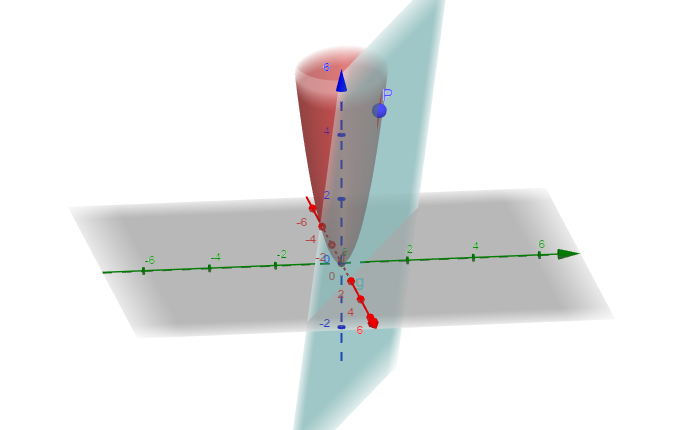
\includegraphics[scale=0.4]{ej10/resources/10.png}  $

\end{document}
